% Note: Ferguson:2007a is "Evidence for publication bias"; Ferguson:2007b is "Good Bad and Ugly: Meta-analytic review"

% Bibtex is screwing up the AAP public policy statement citation. Also Konijn et al.

\documentclass[man]{apa6}
%\documentclass{article}
\usepackage[natbibapa]{apacite}
\usepackage[longnamesfirst]{natbib}
\usepackage{pdflscape}
\usepackage{rotating}
\usepackage{csquotes}
\usepackage{hyperref}

\rightheader{Overestimated Effects of Violent Games}
\shorttitle{Overestimated Effects of Violent Games}

\leftheader{Hilgard et al.}

\threeauthors{Joseph Hilgard}{Christopher R. Engelhardt}{Jeffrey N. Rouder}

\title{Overestimated Effects of Violent Games on Aggressive Outcomes in Anderson et al. (2010)}

\threeaffiliations{University of Pennsylvania}{CARFAX, inc.}{University of Missouri}

\authornote{
Joseph Hilgard, University of Pennsylvania.
Please direct correspondence regarding this article to Joseph Hilgard. E-mail: jhilgard@gmail.com

We thank Randy McCarthy and Katie Corker for suggestions on an earlier draft of this manuscript.

THIS MANUSCRIPT HAS NOT BEEN PEER-REVIEWED. DO NOT CITE WITHOUT THE PERMISSION OF THE CORRESPONDING AUTHOR.}

\abstract{Violent video games are theorized to be a significant cause of aggressive thoughts, feelings, and behaviors.  Important evidence for this claim comes from a large meta-analysis by Anderson and colleagues (2010) that found effects of violent games in experimental, cross-sectional, and longitudinal research. In that meta-analysis, the authors argued that there is little publication or analytic bias in the literature, an argument supported by their use of the trim-and-fill procedure. However, there are now more sophisticated methods than trim-and-fill for the detection of, and adjustment for, publication bias.
In the present manuscript, we re-examine their meta-analysis and apply these new techniques for detecting bias and adjusting effect sizes. 
Our conclusions differ markedly from those of Anderson and colleagues in three salient ways. First, we detect significant publication bias in experimental research. Second, experiments meeting these authors' criteria for methodological quality do not find larger adjusted effects than other experiments, but instead represent a subsample of experiments in which statistical significance was found. After adjusting for bias, there is often little difference between the two estimates. Finally, after accounting for publication bias, effects of violent games on aggressive behavior in experimental research are estimated as being very small, and estimates of effects on aggressive affect are much reduced. 
In contrast, the cross-sectional literature finds correlations that are relatively robust to adjustments for small-study effects.
We outline future directions for stronger experimental research.
The results indicate the need for an open, transparent, and pre-registered research process to test the existence of the basic phenomenon.
}

\begin{document}
\maketitle

Do violent video games make their players more aggressive? Given the continued popularity of violent video games and their increasing technological sophistication, even modest effects of violent games could have serious implications for public health. Psychological research provides evidence of such a link, leading professional organizations to issue policy statements describing harmful effects of violent media (AAP, 2009; APA, 2015). In the view of the professional task forces reviewing the evidence and drafting these statements, the evidence is clear enough, and the hazards certain enough, that the public should be informed and educated of the harmful effects of violent video games. \nocite{APA:2015,AAP:2009}

Despite decades of research and hundreds of studies, however, the basic phenomena remain debated.  For proponents, the effects are obvious, robust, and nearly ubiquitous. For skeptics, the research is not as clean nor the effects as obvious as has been presented.  Instead, skeptics point to a host of issues including construct validity, null findings, and publication bias as undermining the evidence for violent game effects.

The proponents' argument is advanced by a meta-analysis from \citet{Anderson:etal:2010}.  This meta-analysis covers 381 effect-size estimates based on 130,296 participants.  The covered studies were separated into ``best-practices'' and ``not-best-practices'' subsets according to whether they met a set of inclusion criteria. The authors emphasize the best-practices subset, but provide analyses of the full sample as a sensitivity analysis. They find that in best-practices experiments there are statistically and practically significant effects of video game violence on aggressive thoughts ($r = .22$),  aggressive feelings ($r = .29$), and aggressive behaviors ($r = .21$).  Moreover, these effects are not limited to experiments but are also found in cross-sectional comparisons and even in longitudinal research designs. 
Anderson et al. applied the trim-and-fill procedure \citep{Duval:Tweedie:2000} to detect and adjust for publication bias. This procedure recommended minimal adjustment, suggesting that the research literature was only minimally contaminated by publication bias.
\citet{Bushman:etal:2010} and \citet{Huesmann:2010} call the evidence in this corpus of studies ``decisive.'' 

Despite this meta-analysis, there are still skeptics of causal effects of violent video games on aggressive outcomes.  \citet{Ferguson:Kilburn:2010}, for example, are concerned that the \citet{Anderson:etal:2010} meta-analysis may suffer from biases in the publication of studies, the entry of effect sizes into meta-analysis, and the application of the best-practices inclusion criteria.  Other skeptics, such as \citet{Elson:etal:2014}, are also concerned that the individual studies suffer from questionable research practices such as the selective report of dependent variables that yield statistical significance. 
Skeptics suspect that these meta-analytic biases and questionable research practices may overestimate the strength of evidence for, and magnitude of, violent video game effects, despite the results of trim-and-fill analysis.

To address this continued skepticism, we re-analyze the meta-analysis of \citet{Anderson:etal:2010}. We feel this re-analysis is necessary for several reasons:  First, the topic is important and controversial. Effects of violent video games are hotly debated and have implications for public health and for freedom of expression alike. Second, the \citet{Anderson:etal:2010} meta-analysis is a tremendous volume of work encompassing many studies. We were drawn to the quality and quantity of data. Third, there are promising new techniques for addressing potential publication bias and questionable research practices. These new techniques, including PET \citep[Precision-Effect Test,][]{Stanley:Doucouliagos:2014}, PEESE \citep[Precision-Effect Estimate with Standard Error,][]{Stanley:Doucouliagos:2014}, $p$-curve \citep{Simonsohn:etal:2014,Simonsohn:etal:2014b}, and $p$-uniform \citet{vanAssen:etal:2015} may provide better adjustments for these potential artifacts than the method used in \citet{Anderson:etal:2010}. 

\subsection{Concerns About Bias}
We were concerned about three potential sources of bias in the Anderson et al. meta-analysis. The first, {\em publication bias}, is the phenomenon that studies with statistically significant (e.g., $p<.05$) findings are more likely to be submitted and accepted for publication than are studies with non-significant results. The second, {\em $p$-hacking}, is the possibility that researchers increase their Type I error rates in an attempt to find publishable, statistically significant results. The last, {\em selection bias}, is the application of flexibility in meta-analytic inclusion criteria. We discuss each in turn.

\subsubsection{Publication bias}
Publication bias is a problem that contributes to the overestimation of effect sizes and the propagation of Type I error. When studies that attain statistical significance are more likely to be published than those that are not, meta-analyses of the published literature are no longer representative of the full body of research. Note that publication bias is proportionate, not absolute. The presence of some published null results therefore does not rule out the possibility of any publication bias. Note also that the bias can be inflicted at both the level of journals, which may reject null results, and authors, who may not bother submitting null results.
Meta-analyses of literatures suffering from publication bias are likely to overestimate effect sizes and may reach incorrect conclusions of statistically and practically significant effects.

The critical question is whether there is evidence for publication bias in the violent video-game literature as synthesized by \citet{Anderson:etal:2010}.  Here there is disagreement.  Anderson et al. claim that there is little evidence for publication bias.  Their claim follows from their attempts to account for such bias using both statistical methods and literature review.  

With regard to statistical methods, the authors used a trim-and-fill procedure to estimate bias-adjusted effect size estimates. This procedure recommended only a small adjustment, thereby suggesting a minimal degree of publication bias. This claim has two weaknesses. First, although it was state-of-the-art at the time of the Anderson et al. analysis, the trim-and-fill correction is understood today to be somewhat ineffective. It corrects for bias when bias is absent and does not correct enough when bias is strong \citep{Simonsohn:etal:2014b,vanAssen:etal:2015}. It also has difficulty adjusting effect sizes to zero when the null is true and there is publication bias \citep{Moreno:etal:2009,vanAssen:etal:2015}. 
% \citet{Ferguson:2007} applied a different test for publication bias and found signs of publication bias in the literature, but \citet{Anderson:etal:2010} argue that the application of the test was weakened by a less-than-comprehensive literature search.

With regard to literature review, the authors made an attempt to collect unpublished literature. The authors found 18 dissertations that had gone unpublished, 16 of which failed to find statistical significance on one or more outcomes. Only one unpublished non-dissertation study was found. We suspect that, despite the authors' efforts, there may be more unpublished non-dissertation studies censored from report. On this basis, more detailed consideration of the possibility of bias in the Anderson et al. meta-analytic dataset is warranted.

\subsubsection{$p$-hacking}
Because statistically significant results are easier to publish, particularly in prestigious journals, researchers often strive for statistical significance. Often, this striving leads to the desired statistical significance but also causes an inflated Type I error rate; the obtained result is more likely to be a false positive. Practices that lead to this inflation of Type I error include data-dependent stopping (i.e., deciding to end data collection when $p < .05$ or continue when $p > .05$), the strategic inclusion or exclusion of outliers depending on their influence on the results, or the analysis of subgroups when the full sample fails to detect an effect. Another form of $p$-hacking is outcome switching: If an experiment's primary outcome does not find the desired result, other outcomes with more statistically significant changes might be presented instead and the primary outcome hidden from report.

It has been argued that such outcome-switching may exist in the quantification and report of certain measures of aggressive behavior. Some researchers measure aggressive behavior by allowing participants to administer a painful burst of noise to another participant. Both the volume and duration of such a noise burst are measured.  There is considerable diversity in the way studies have combined these quantities, and \citet{Elson:etal:2014} suggest that this diversity reflects the fact that some studies find statistical significance under one combination while other studies find significance under a different combination.  In general, when researchers collect several dependent measures, there exists the possibility that there is some strategic selection among them. Such selection of the larger, more statistically significant outcomes risks overestimation of the net effect size. 

\subsubsection{Selection bias}
Selection bias may contaminate meta-analysis when the researchers include or exclude studies on the basis of the hypothesis they favor. In that regard, the application of the best-practices inclusion criteria applied by Anderson et al. was the subject of some controversy. \citet{Ferguson:Kilburn:2010} argued that the inclusion criteria were applied more liberally to studies with significant results than to studies with nonsignificant results. If this is the case, then the best-practices subset may find larger effects not due to stronger methodology, but because of greater overestimation through selection bias. 

\subsection{Assessing Bias in Meta-Analysis}
There are several approaches to assessing the aforementioned biases in meta-analysis. Some of these are recent developments published only after the publication of \citet{Anderson:etal:2010}. We used these tests and methods to provide further analysis of the Anderson et al. meta-analysis. Additionally, we looked at the corpus of dissertations not published in journals and considered how their estimates differed from other collected research.

\subsubsection{Statistical Procedures}
A common theme in many statistical tests for meta-analytic bias is the relationship between effect size and precision (or sample size) in reported studies. In an unbiased research literature, there should be no relationship between effect size and precision; sample size does not cause effect size. However, such a relationship will be observed if publication favors statistically-significant studies at the expense of nonsignificant studies. Small-sample studies need large observed effect sizes to reach statistical significance, whereas large-sample studies can reach statistical significance with smaller observed effect sizes. Thus, in the presence of publication bias, there is an inverse relationship between effect size and precision. 

One critical issue in meta-analysis in general, and the relationship between effect size and precision in particular, is whether the combined studies are similar enough to each other that synthesizing them is reasonable. When studies are similar, they are said to be homogeneous; when they are dissimilar, they are said to be heterogeneous.
Meta-analysts seek to minimize the extent of heterogeneity by dividing studies into roughly homogeneous subgroups based on their methodologies, study populations, and other features. Despite these efforts, results can nevertheless be inconsistent across studies, and conclusions must consider the challenges of heterogeneity. Heterogeneity can be estimated statistically by examining whether the variance between studies exceeds what would be expected by sampling error alone. Most of the bias-adjustment methods below assume homogeneity, and all will have difficulty in the face of substantial heterogeneity.    

Sometimes heterogeneity can cause a correlation between sample size and effect size that is not due to bias. For example, experimental studies tend to have smaller samples than cross-sectional studies, and each paradigm may reflect different underlying effect sizes. Alternatively, it may be possible that manipulations and measurements in small samples are more effective than in large samples. If effect sizes are heterogeneous and researchers are performing {\em a priori} power analyses, there will be a relationship between sample size and effect size that does not represent bias in research.
To represent these possibilities, relationships between sample size and effect size are often called ``small-study effects'' rather than ``publication bias.'' Some of these possibilities can be excluded through practice. For example, conducting separate bias tests for cross-sectional and experimental studies can rule out study design as a potential cause of small-study effects.

\paragraph{Funnel plots}
Funnel plots provide a useful graphical summary of potential small-study effects in meta-analysis.  The relationship between effect size and sample size is plotted, allowing for visual estimation of small-study effects. In a funnel plot, effect size is plotted on the $x$-axis and precision on the $y$-axis. In the absence of small-study effects and heterogeneity, study results will form a symmetrical funnel shape, displaying substantial variance when sampling error is large but narrowing to a precise estimate when sampling error is small. Because of this sampling error, some small-sample studies are expected to find null or even negative results even when the underlying effect is positive, so long as there is not bias. 

Such symmetry is not found in funnel plots of research contaminated with publication bias or $p$-hacking.  In the case of publication bias, studies are missing from the lower portion of the funnel where results would not reach statistical significance. This asymmetry can also be caused by $p$-hacking. When samples are collected until a desired $p$-value is attained, published studies will increase in both precision and effect size, moving towards the upper-right edge of the funnel. When subgroups or experimental subgroups are dropped from report to highlight only a subgroup in which statistical significance was found, studies will lose precision and increase in effect size, moving towards the lower-right edge of the funnel. When outcomes are censored from report to highlight only the significant outcomes, the effect size increases, moving studies to the right of the funnel. 

Under conditions of heterogeneity, funnel plots may overestimate the degree of asymmetry \citep{Lau:etal:2006,Terrin:etal:2003}. Variability among studies may cause some precisely estimated studies to have effect size estimates far from the overall mean, giving the false impression of small-study effects. For this reason, homogeneity is desired for tests and adjustments related to the funnel plot.

One of the critical issues in meta-analysis is what may be learned in the presence of bias. The most charitable position is that researchers may assess the degree of bias and provide needed corrections to recover accurate effect size estimates \citep[e.g.,][]{Duval:Tweedie:2000,Simonsohn:etal:2014b}.  We are less sanguine, as much is unknown about the statistical properties of corrections---their efficiency and bias in realistically-sized samples as well as their robustness to violations of assumptions.  Still, they have some value in analysis. We provide a review of the bias-detection-and-correction methods used in this study, noting the strengths and weaknesses of each. 

\paragraph{Egger's regression test}
Egger's weighted regression test \citep{Sterne:Egger:2005} inspects the degree and statistical significance of the relationship between sample size and effect size. A significant test statistic suggests that the observed funnel plot would be unusually asymmetrical if the collected literature were unbiased. This test is sometimes helpful in reducing the subjectivity in visually inspecting a funnel plot for asymmetry. 

Egger's regression test has some weaknesses. Although it can detect bias, it does not provide a bias-adjusted effect size. The test is also known to have poor statistical power when bias is moderate or studies are few, limiting the strength of conclusions that can be drawn through application of the test \citep{Sterne:etal:2000}. Performance is also likely to degrade under conditions of heterogeneity \citep[e.g.,][]{Lau:etal:2006,Terrin:etal:2003}. Skeptics have used Egger's test to look for bias in the violent-game-effect literature \citep[e.g.,][]{Ferguson:2007,Ferguson:Kilburn:2009}, but \citet{Anderson:etal:2010} abstained from its use. 

\paragraph{Trim and fill}
One popular bias-adjustment technique, trim and fill \citep{Duval:Tweedie:2000}, is used to detect and adjust for bias through inspection of the number of studies with extreme effect size estimates on either side of the meta-analytic mean estimate. If the funnel plot is asymmetrical, the procedure ``trims'' off the most extreme study and imputes a hypothetical censored study reflected around the funnel plot's axis of symmetry (e.g., an imputed study with a much smaller or even negative effect size estimate). Studies are trimmed and filled in this manner until the ranks are roughly equal. 

% TODO: Other citations for criticism of trim-and-fill?
% TODO: COnsider citing Peters, Sutton, Jones, Abrams, & Rushton, 2007
% TODO: Consider citing Nik Ruzni Nik Idris, 2011, Am Journal of Applied Sciences
% TODO: Consider adding Terrin et al. 2003 to this

Trim-and-fill has its critics.  \citet{Moreno:etal:2009}, \citet{Simonsohn:etal:2014b}, and \citet{vanAssen:etal:2015} argue it is not useful: when there is no bias, there is too much adjustment, and when there is strong bias, there is too little adjustment. Higgins and Green (2011) express concern about the imputation of studies, which adds purely hypothetical data to the meta-analysis. Finally, as with most adjustments for bias, trim-and-fill performs best when studies are homogeneous. \citet{Terrin:etal:2003} point out that heterogeneity may degrade trim-and-fill's performance considerably. % TODO: Any specific degredation?
\nocite{Higgins:Green:2011}
% Cochrane Handbook for Systematic Reviews of Interventions, March 2011, v5.1.0) %url: http://handbook.cochrane.org/chapter_10/10_4_4_2_trim_and_fill.htm

For these reasons, trim-and-fill is most commonly suggested as a form of sensitivity analysis rather than a serious estimate of the unbiased effect size. When the na{\"i}ve meta-analytic estimate and the trim-and-fill-adjusted estimate differ only slightly, it is suggested that the research is largely unbiased; when the difference is large, it suggests potential research bias.
\citet{Anderson:etal:2010} applied the trim-and-fill procedure in their meta-analysis. The procedure yielded only slightly-adjusted effect sizes, and so the authors concluded minimal research bias.
Again, the development of novel adjustments for small-study effects allows for further testing of this conclusion.

\paragraph{PET and PEESE meta-regression}
Meta-regression is a promising new tool in bias detection and adjustment. Meta-regression estimates a bias-adjusted effect size by considering the relationship between effect size and precision, then estimating the underlying effect size that would be found with perfect precision. Two meta-regression estimators are the Precision-Effect Test (PET) and Precision-Effect Estimate with Standard Error (PEESE) \citep{Stanley:Doucouliagos:2014}. 

In PET, a weighted {\em linear} regression is fit to describe the relationship between effect size and precision, as in the Egger regression test. Unlike Egger's test, however, PET then extrapolates from this regression to estimate what the effect would be in a hypothetical study with perfect precision. When there is minimal bias, there is minimal adjustment. When there is no underlying effect, published studies tend to lie on the boundary between statistical significance and nonsignificance, forming a linear relationship between sample size and precision. Thus, PET performs well at estimating effects when the underlying effect is approximately zero. However, PET performs less well when there is some effect. When there is an underlying effect, small studies will be censored by publication bias, but most large studies will find statistical significance and be unaffected by bias. PET will fail to model this nuance and risks underestimating the size of nonzero effects \citep{Stanley:Doucouliagos:2014}.

A second meta-regression estimator, PEESE, is intended to address this problem. PEESE fits a weighted {\em quadratic} relationship between effect size and precision. The resulting curve models bias as being stronger in the lower part of the funnel but reduced as the studies become better-powered and less subject to censoring. Again, in the absence of bias, adjustment is minimal. PEESE is less likely than PET to underestimate nonzero effects, but risks overestimating the size of null effects \citep{Stanley:Doucouliagos:2014}.

Because PET underestimates nonzero effects and PEESE overestimates null effects, sometimes PET and PEESE are combined as a two-step conditional PET-PEESE procedure. If PET detects a significant effect, the PEESE estimate is used; if PET does not detect a significant effect, the PET estimate is used. Although this approach would seem to make use of the estimators' complementary strengths and weaknesses, this approach may be exceedingly conservative, as PET has questionable statistical power for the detection of effects \citep{Gervais:2015}. When PET's power is poor, conditional PET-PEESE tends to underestimate effects, as only PET is ever applied. For this reason, we report both PET and PEESE. When the PET estimate is significant, the PEESE estimate should be favored, but when it is not significant, one should not necessarily favor PET over PEESE, as non-significant results do not guarantee the truth of the null hypothesis. Caution is also necessary in conditions of heterogeneity, under which the performance of PET and PEESE will degrade.

These meta-regression techniques have been previously applied by \citet{Carter:McCullough:2014} to inspect the amount of evidence for ``ego depletion,'' the phenomenon of fatigue in self-control. They found that after adjusting for small-study effects, PET-PEESE suggested an absence of evidence for the phenomenon. The authors therefore recommended a large-sample pre-registered replication effort, which found no evidence of ego depletion \citep{Hagger:etal:inpress}.

\paragraph{$p$-Curve}
Another novel technique for accounting for small-study effects is $p$-curve \citep{Simonsohn:etal:2014,Simonsohn:etal:2014b}. The $p$-curve technique estimates the underlying effect size by inspecting the distribution of significant $p$-values. 
When the null hypothesis is true (i.e. $\delta$ = 0), the $p$-curve is flat: significant $p$-values are as likely to be less than .01 as they are between .04 and .05. When the null hypothesis is false, the $p$-curve becomes right-skewed such that $p$-values less than .01 are more common than are $p$-values between .04 and .05. The degree of right skew is proportionate to the power of studies to detect an effect; larger sample sizes or effects will yield greater degrees of right skew. By considering the $p$-values and sample sizes of significant studies, $p$-curve can be used to generate a maximum-likelihood estimate of the true effect size.

One weakness of $p$-curve estimation is that questionable research practices introduce left skew into the $p$-curve. The combination of right skew from fairly reported studies and left skew from questionable studies results in a flatter $p$-curve than would be found if all studies had been fairly reported. Thus $p$-curve will underestimate the true effect size in these circumstances. Aside from this weakness, simulation work suggests that $p$-curve is quite effective at estimating true effect sizes \citep{Simonsohn:etal:2014,Simonsohn:etal:2014b}.  Another weakness of $p$-curve is that studies with $p$-values above the .05 criterion are not considered, resulting in a substantial loss of information.  Consequently, the approach can be inefficient, especially when effect sizes are small or statistical significance is rare.  

In contrast to the funnel-plot-based tests and estimators, which are derived from the relationship between sample size and effect size, $p$-curve is a function of statistical power. Thus, these estimators will perform differently given heterogeneous effect sizes and {\em a priori} power analysis. Whereas funnel plots will detect small-study effects in this scenario, spuriously suggesting research bias, $p$-curve will find that the significant studies are appropriately powered.\footnote{See supplementary file p\_curve\_power\_analysis.R for a simulation.}

Heterogeneity can nonetheless influence effect size estimation using $p$-curve. $P$-curve considers only the statistically significant results, and studies with greater underlying effect sizes are more likely to attain statistical significance. This can cause $p$-curve to estimate a larger effect size than does na{\"i}ve meta-analysis, as the na{\"i}ve analysis considers all studies, whereas $p$-curve considers only the statistically-significant ones. 

\subsubsection{$p$-uniform}
$P$-uniform is another power-based test and adjustment for bias \citep{vanAssen:etal:2015}. Like $p$-curve, it considers only the statistically-significant results in meta-analysis. It attempts to find an underlying effect size for which the conditional $p$-value distribution would be as close to uniform as possible. That is, it looks for an effect size $\delta_0$ for which the null hypothesis $H_0: \delta = \delta_0$ would generate an approximately uniform distribution of $p$-values. It also provides a test for publication bias by considering whether the adjusted effect size is statistically significantly smaller than the na{\"i}ve meta-analytic estimate. Like $p$-curve, it only considers studies with $p < .05$, and so may lose substantial information. It also assumes a fixed effect size and so may perform poorly under conditions of heterogeneity.   

\subsubsection{Test for Excess Significance}
Another power-based test for publication bias is the Test for Excess Significance \citep{Ioannidis:Trikalinos:2007}. This test estimates the number of expected studies with statistical significance given some anticipated effect size (usually the na{\"i}ve meta-analytic estimate), then compares that expectation against the number of observed significant results. A significant test suggests censoring of nonsignificant results or the manipulation of results into statistical significance.

This test has a number of weaknesses. It has poor statistical power \citep{Ioannidis:Trikalinos:2007}, and the validity of its $p$-value rests on strong, perhaps unwarranted assumptions about researcher behavior \citep{Morey:2013}. Like other tests for bias, its results may be spurious when there exists genuine between-study heterogeneity. We report the test for completeness, but the reader is urged to interpret the result with considerable caution.

\subsubsection{Unpublished Dissertations}
Yet another approach is to eschew statistical adjustments and attempt to inspect the unpublished literature directly. When unpublished work provides smaller effect size estimates than published work, publication bias may be present.
Nonsignificant results can be difficult to retrieve for meta-analysis as they often go unpublished and forgotten. However, one publication format is largely immune to these publication pressures: the doctoral dissertation. Department requirements generally dictate that dissertations be submitted and published in a dissertation database regardless of whether or not that dissertation is later published as a peer-reviewed journal article.  Another advantage of dissertations is that they are typically thorough, reporting all outcomes and manipulations, whereas published journal articles may instead highlight only the significant results \citep{O'Boyle:etal:2014}. Dissertations, then, provide us with a sample of reported studies relatively uncontaminated by publication biases favoring significant results. Anderson and colleagues did an excellent job of retrieving unpublished dissertations for their meta-analysis. In our analyses, we examine these unpublished dissertations and the statistical significance of their results.

\subsection{Summary of Methods}
Given this state of the field, our analysis will consist of two main questions.  First, is there evidence of small-study effects in the dataset?  The presence or absence of these effects will be assessed informally by inspection of funnel plots and more formally by the Egger test. Supplementary tests will be provided by $p$-uniform and the Test for Excess Significance.  Second, what might be appropriate bias-adjusted estimates?  We will apply PET, PEESE, $p$-curve, and $p$-uniform to estimate bias-corrected effect sizes.  The answer to this second question is necessarily tentative because the statistical properties of these adjustments are only coarsely known. Finally, we will consider whether there are differences between the results of published articles and unpublished dissertations that might suggest bias.

\section{Method}
We perform a reanalysis of the \citet{Anderson:etal:2010} meta-analysis using the data as provided by the study's first author.  We augment the trim-and-fill approach with funnel plots, PET and PEESE meta-regression, $p$-curve and $p$-uniform analyses, and the Test for Excess Significance. We use the original authors' separation of studies by study design (experimental, cross-sectional, longitudinal), by study outcome (affect, behavior, cognition, arousal), and by study quality (all studies, best-practices subset) in our presentation. Thus, point-biserial correlations from experiments and product-moment correlations from cross-sections are treated separately, as is generally preferred. Finally, we perform $\chi^2$ tests to see whether unpublished dissertations are more or less likely to yield statistical significance than other published work.

In the original dataset, \citet{Anderson:etal:2010} coded all effect sizes in terms of Pearson $r$, then converted these to Fisher's $z$-scores with standard error of $1/\sqrt{N-3}$. This approach is appropriate given that most outcome measures are either continuous or at least modeled as continuous by study authors. We use their estimated $z$-scores and standard errors in this analysis. This approach has the benefit of providing standard errors that are not a function of effect size. Standard errors that are a function of their corresponding effect sizes can lead to the spurious detection of small-study effects.

Our inspection focuses on the raw effect sizes contained in that report. Anderson and colleagues report partial correlation coefficients for cross-sectional studies; we abstain from analysis of these. Re-analysis of the partial effect sizes is likely to be challenging due to the particularities of partial correlations \citep[see, e.g.,][]{Aloe:2014} and as such is omitted from the current manuscript.

All data and code have been made available online at \url{https://osf.io/r76j2/?view\_only=0cbfaef76d0142c0864de9f28a4324e1}. We thank Dr. Anderson for sharing with us the dataset from \citet{Anderson:etal:2010} and inviting us to host it publicly. 

\subsection{Aggregation within Studies}
As we apply them, the meta-analytic procedures assume that entire studies are censored or re-analyzed per their statistical significance. However, the original data have some studies divided into subsets to test for moderators. For example, one study might be entered as two records: one for the simple effect among males, and another for the simple effect among females. Where multiple effects were entered for a single study, we aggregated these to form a single effect size estimate by summing the sample sizes and making a weighted average of the subsample effect sizes. This parallels the behavior of the software used in the original analysis. 

\subsection{Calculation of $p$-values}
Although the original data entry performed by Anderson and colleagues is admirably thorough, the data set given us does not have the necessary statistics for $p$-curve meta-analysis. We calculated $t$-values by the equation $r \times \sqrt{\frac{n-2}{1-r^2}}$, then used the $t$-value to calculate a two-tailed $p$-value. We do not report a $p$-value disclosure table as recommended by \citet{Simonsohn:etal:2014}, as the meta-analyzed $p$-values are a function of the data as entered by Anderson et al. and not a direct entry of $p$-values from manuscripts.
Note that the $p$-values we enter thereby correspond to the main effect of violent video game exposure as entered by Anderson et al. and not the specific hypothesis tests conducted or reported by the studies' original authors.

\subsection{Adjusted Estimates}
PET was performed by fitting a weighted-least-squares regression model predicting effect size as a linear function of the standard error with weights inversely proportional to the square of the standard error. PEESE was also performed, predicting effect size as a quadratic function of the standard error and using similar weights. All meta-regressions were performed using the \texttt{metafor} package for {\bf R} (Viechtbauer, 2010), using the {\tt rma()} function to fit a weighted random-effects model with an additive error term. Models were fitted via restricted maximum-likelihood (REML) estimation, per package defaults. Effect sizes are converted from Fisher's $z$ to Pearson $r$ for tables and discussion. 
\nocite{Viechtbauer:2010} 

For $p$-curve, we used the R code behind version 3.0 of the online $p$-curve app \citep{Simonsohn:etal:2014}, entering a $t$-value and degrees of freedom parameter for each relevant study.  This code provides estimates in terms of Cohen's $d$. We converted these to Pearson $r$ for consistency of presentation, using the formula $\frac{d}{\sqrt{d^2+4}}$. Full $p$-curve output from the online p-curve.com application is available in the supplementary materials

For $p$-uniform, we use the \texttt{puniform} package provided by van Aert at \url{https://github.com/RobbievanAert/puniform}. Analysis was performed using the correlations and sample sizes as entered by Anderson et al. The package's default method for the aggregation of $p$-values was used. % Reference entry needed for the software package? Seems that citing the p-uniform paper is good enough.

PET, PEESE, and $p$-curve are likely to perform poorly when there are few datapoints. Therefore, our analyses are restricted to effects and experimental paradigms with at least ten independent effect sizes. %citation may be needed from Carter & McCullough, 2014
Readers who want to generate estimates for more sparse datasets or explore the impact of our inclusion and exclusion decisions are invited to download the data and code.

\subsubsection{Sensitivity analysis}
In addition to our analysis of the full dataset as provided by Anderson and colleagues, we perform leave-one-out sensitivity analyses, removing each datapoint one at a time and making all adjusted estimates. A supplementary spreadsheet is attached that lists the individual studies and the estimates when they are left out.\footnote{Initially, we had attempted a different sensitivity analysis in which we removed datapoints with a Cook's distance of more than 0.5 on the PET regression. In the case that several observations were excessively influential, we performed an iterative procedure, deleting the single most influential observation and checking again for influence until no observations had excessive influence. In practice, this tended to delete all datapoints that did not fit the PET regression well. This seemed to inappropriately favor the PET model over the available data, so we abandoned this approach.}

\subsection{Studies Excluded}
We removed three studies from meta-analysis due to concerns over relevance and accuracy. First, \citet[study 1]{Matsuzaki:etal:2004} was removed because its entered effect sizes were unusually large for their precision (i.e., aggressive behavior $r = .60$ and aggressive cognition $r = .53$), were highly influential on the meta-regression model, and could not be found as entered in the \citet{Anderson:etal:2010} dataset by inspection of the original article. %\footnote{We asked Dr. Anderson for comment. He replied, ``The Japanese team reported additional results for a number of their papers, in those cases in which the initial paper didn't have what was needed. This was true for several other papers as well. For example, if an original paper reported only some composite measure of aggressive personality but had more specific data on physical aggressiveness, we tried to get the more appropriate measure.'' It seems unlikely to us that such a large effect would be found on a single most-appropriate measure and nevertheless would go unreported in favor of a smaller composite effect. However, it is certainly possible. Without recourse to the raw data, we omit this study as an outlier and probable error of data entry.} 
\citet{Panee:Ballard:2002} was removed because the study tested the effects of violent primes on in-game behaviors, not the effects of violent gameplay on aggressive outcomes; therefore, it does not provide a relevant test of the hypothesis. 
Finally, \citet{Graybill:etal:1985} was removed from analysis. As entered in the Anderson et al. dataset, the effect size was unusually large and significant, $r = 0.57, p = 1.6 \times 10^{-10}$. The cause of this enormous outcome was that the study's manipulation checks were entered as though they were primary study outcomes on aggressive cognitions; again, this is not a relevant hypothesis test. 

\subsection{Subsets Re-analyzed}
We reproduce estimates from \citet{Anderson:etal:2010} and apply PET, PEESE, $p$-curve, and $p$-uniform to detect and adjust for small-study effects. Sufficient datapoints were available to re-analyze experimental studies of aggressive affect, aggressive behavior, aggressive cognition, and physiological arousal, as well as cross-sectional studies of aggressive affect, aggressive behavior, and aggressive cognition. Studies are further divided to create separate best-practices-only and all-studies estimates per \citet{Anderson:etal:2010} as sample sizes permit. 

The numbers of studies, overall numbers of participants, and na{\"i}ve fixed- and random-effects estimates are provided for each subset in Table~\ref{table:naive}.

\section{Results}
Again, we wished to know whether there are small-study effects indicative of bias, and if so, what are appropriate bias-adjusted effect size estimates. We present each in turn.  

\subsection{Detection of Bias}
The first question is addressed by inspection of the funnel plots in Figures \ref{funnel-aggaff}, \ref{funnel-aggbeh}, \ref{funnel-aggcog}, and \ref{funnel-physarous}.  Here we see dramatic funnel-plot asymmetry in several conditions. Application of best-practices criteria did not ameliorate this asymmetry. Asymmetry is present, and sometimes stronger, in many best-practices subsamples.

This funnel-plot asymmetry was tested by Egger's regression. Results are provided in Table \ref{table:Egger}. 
The regression test for funnel-plot asymmetry was statistically significant in several subsets of the data. Funnel plots were significantly asymmetrical in all analyses of cross-sectional research: affect, behavior, and cognition, both best-practices and full-sample sets. Heterogeneity, however, may limit the strength of this finding. There was also significant asymmetry in both sets of experiments studying aggressive affect.
Notably, the Egger test was not significant in the full sample of experiments of aggressive behavior, but it was in the best-practices subsample, suggesting that the application of best-practices inclusion criteria may have exacerbated funnel-plot asymmetry. On the other hand, the full sample of experiments of physiological arousal was significantly asymmetric, whereas the best-practices subsample was not.

The Test of Excess Significance suggested an excess of significant results in the full sample of experiments of aggressive affect, the full sample of experiments of aggressive behavior, and the best-practices subsample of experiments of aggressive behavior. $P$-uniform suggested significant bias only for experiments of aggressive behavior, both for the full sample and for the best-practices subsample.
% TODO: Report full set of statistics in a table.
% TODO: Point out any cases where I^2 was large enough that I should be concerned.

In total, these results indicate that small-study effects are likely present in studies of violent game effects. Such a result is concerning because it indicates that the collected meta-analytic data may be contaminated by publication, analytic, or selection biases, and may therefore yield biased overestimates of effect sizes.

\subsection{Adjusted Effect Sizes}
% TODO: Add $p$-uniform output to this table and this section
% TODO: Consider separate tables for separate estimators.
Results of the $p$-curve, $p$-uniform, PET, and PEESE analyses are provided in Table \ref{table:adjustment}. We caution the reader that we do not know the small-sample properties of the adjusted estimators and so do not valorize one in particular as being likely to provide the most accurate estimate of the underlying effect. Instead, we consider all estimators and look for convergence among adjusted estimates. Like Anderson et al., we will emphasize in this text the results of the analysis of the best-practices subsample.

Among experimental studies, the estimators yield larger adjustments for bias than did Anderson et al.'s trim-and-fill estimators. In general, PET and PEESE suggested substantially lower effect sizes in experimental research, whereas $p$-curve and $p$-uniform suggested smaller adjustments. The notable exception is experiments of aggressive behavior, in which $p$-curve and $p$-uniform adjusted as harshly as did PET.

% When excluding Ballard & Wiest (1999), best-practices: naive FE, r = .27, naive RE r = .27, puniform r = .20, p-curve r = .19, PET r = -.01, PEESE r = .17; full sample: naive FE r = .16, naive RE r = .18, PET r = -.035, PEESE r = .09, puniform r = .21, pcurve r = .19
In experiments of aggressive affect, the original report suggested no adjustment was necessary for the best-practices subset. By contrast, our analyses suggested downward adjustments. Relative to the fixed-effects estimate, $p$-uniform suggested an adjustment of -.05 to $r$ = .24, and $p$-curve suggested an adjustment of -.08 to $r$ = .21. PEESE adjusted by -.15 to $r$ = .14, and PET adjusted the effect into nonexistence ($r$ = -.12). Exclusion of an outlier \citep{Ballard:Wiest:1996} reduced the na{\"i}ve estimates ($r$ = .27, fixed- and random-effects), the $p$-uniform estimate ($r$ = .20), and the $p$-curve estimate ($r$ = .19). This exclusion also increased the PET ($r$ = -.01) and PEESE ($r$ = .17) estimates. Thus, exclusion of the outlier seems to have brought the adjustments into greater agreement.

In experiments of aggressive behavior, the original report suggested an adjustment of -.03 to $r$ = .18. By contrast, our analyses recommended harsh downward adjustments ranging from -.06--.19, reducing $r$ to .15 (PEESE) or as little as .02 ($p$-uniform). Our analyses also contest Anderson et al.'s conclusion that studies in the best-practices subsample find larger effects than do the not-best-practices studies. PEESE, $p$-uniform, and $p$-curve suggested identical estimates for the full sample and the best-practices subsample, whereas PET suggested that the effect was larger in the full sample than in the best-practices subsample. 

In experiments of aggressive cognition, the original report suggested an adjustment of -.02 to $r$ = .20. Our adjustments are divergent, perhaps due to the moderate heterogeneity among studies of this outcome. $P$-uniform suggested increasing the estimate by .02 to $r$ = .24, $p$-curve suggested an adjustment of -.03 to $r$ = .19, PEESE suggested adjusting by -.04 to $r = .18$, and PET suggested adjusting by -.12 to $r = .10$.

Estimates of the effects on physiological arousal seemed robust to adjustments for small-study effects. Among the best-practices subset of experiments, PEESE, $p$-curve, and $p$-uniform suggested effects as large as, or larger than, the na{\"i}ve estimate. Again, the presence of moderate heterogeneity may limit the strength of the conclusions possible given the data.

Among cross-sectional studies, our estimators suggested minimal need for adjustment. PEESE, $p$-curve, and $p$-uniform all estimated effect sizes very close to the na{\"i}ve random-effects estimate. This was true even of studies of aggressive behavior, for which Egger's test suggested significant asymmetry in the full-sample analysis. However, the considerable heterogeneity in these subsets may limit the efficacy of these adjustments and may indicate the need for further consideration of differences in study methodology.

Modeling the relationship between sample size and effect size also substantially reduced the heterogeneity in some subsets of the data. Among best-practices experiments of aggressive affect, no heterogeneity remained in the PET and PEESE models. Similar homogeneity was attained among experiments of aggressive behavior in both the best-practices and full samples. This suggests that there is little residual variance in study results to explain by study attributes. In the case of best-practices experiments of aggressive behavior, there was so little residual variance that a confidence interval on $I^2$ could not be calculated. The documentation for \texttt{metafor} suggests that this indicates ``highly (or overly) homogenous data,'' \citep[helpfile for confint.rma.uni]{Veichtbauer:2010} an unusual absence of residual sampling variance. This would be consistent with the presence of bias: effect sizes in this subset seem to reach statistical significance with improbable precision.

By comparison, modest heterogeneity remained among experiments of aggressive cognition and among the full sample of experiments of aggressive affect. Heterogeneity was also present among nonexperimental work, particularly in studies of aggressive affect. More work will be necessary to distinguish those studies finding larger effects from those finding smaller effects.

There are some instances of convergence in our presented estimates. When inspecting effects on aggressive behavior in experiments, $p$-curve, $p$-uniform, and PET estimated that the underlying effects were so small as to be possibly undetectable in typical sample sizes. Notably, these estimates are highly consistent with some recent reports \citep{Engelhardt:etal:2015,Kneer:etal:inpress,Tear:Nielsen:2014,Przybylski:etal:2014}. For effects on aggressive affect and cognitions in experiments, $p$-curve and PEESE yielded similar estimates, suggesting that there may be detectable, nonzero effects despite overestimation. 

% TODO: Consider the extent to which these dissertations had or lacked quality and relevance.
\subsection{Unpublished Dissertations}
The funnel plots previously presented suggest the presence of substantial bias in publication or analysis. If this is the case, then unpublished dissertations may be less likely to have found statistical significance. 

Funnel plots highlighting the unpublished dissertations using experimental paradigms are provided in Figure \ref{funnel-diss}. As one might expect given publication bias, the unpublished dissertations generally populate the left side of the funnel plot. 

We applied $\chi^2$ tests to examine two relationships: First, the relationship between statistical significance and publication status, and second, the relationship between publication status and selection as meeting best-practices criteria. Frequencies are given in Table \ref{table:dissertations}. The liberal counts assume independence of each entered effect size, while the conservative counts aggregate all effect sizes within each study. The aggregation in this latter counting strategy lead to three categories of studies: those that found significance on all outcomes, those that found significance on some outcomes, and those that found significance on no outcomes.

All tests were statistically significant. Unpublished dissertations were much less likely to have found statistical significance than published studies (liberal and conservative tests, $p < .001$).
Similarly, unpublished dissertations were far less likely to be included as best-practices than published studies (liberal test, $p < .001$; conservative test, $p = .003$). 
To the extent that these unpublished dissertations may reflect competent research less influenced by publication pressure, these results may be cause for concern.

Meta-analytic effect size estimates were also drastically reduced within the set of experiments reported in unpublished dissertations. For aggressive affect, the random-effects estimate fell from $r = .22$ [.15, .29] in the full sample to $r = .02$ [-.10, .15] in unpublished dissertations; for aggressive behavior, the estimate fell from $r = .17$ [.14, .20] in the full sample to $r = .01$ [-.11, .12] in unpublished dissertations; and for aggressive cognitions, the estimate fell from $r = .20$ [.16, .24] in the full sample to $r =  .13$ [.02, .24] in unpublished dissertations.  These estimates should cause pause---they indicate that studies failing to find significant evidence for violent-game effects are likely to go unpublished.

% TODO: Consider summarizing all the replies I had to the editor here re: how pub bias and p-hacking may work in this literature: journal prestige, abandoned dissertations, etc.
\section{Discussion}
Our findings differ from those of \citet{Anderson:etal:2010} in three important ways. First, we find strong evidence of publication bias where the original analysis argued minimal bias. The funnel plots appear asymmetrical, application of Egger's test confirms the presence of significant asymmetry, and bias-adjusted estimates were substantially smaller than the na{\"i}ve estimates. Second, the original meta-analysis claimed that methodologically strong experiments found larger effects than did methodologically weak experiments. Instead, we find that best-practices experiments yield adjusted estimates comparable to the full set of experiments. Division of studies into best- and not-best-practices sometimes exacerbated funnel-plot asymmetry, leading to higher na{\"i}ve estimates but comparable adjusted estimates.  
Third, the original meta-analysis argued that all outcomes were statistically and practically significant. In our analysis, we find instead that the effect of violent video games on aggressive behavior in experiments is likely smaller than anticipated, and may be so small as to be very challenging to study ($r$ = .02--.15). If this is accurate, then the average experiment examining aggressive behavior may be seriously underpowered; there may not be much evidence for violent games' effects on aggressive behavior. 

Overestimation seems most clear in experiments of aggressive behavior. By contrast, overestimation is less clear in experiments of aggressive affect and aggressive cognition. With respect to experiments of aggressive affect, the funnel plot is clearly asymmetrical, but our estimators disagree on the degree of bias. Meta-regression suggested effects near zero, whereas $p$-value-based adjustments suggested effects near the na{\"i}ve estimate. With respect to experiments of aggressive cognition, there is less evidence of small-study effects. Nevertheless, there may be some degree of overestimation. To what degree there is overestimation is unclear, as our estimators did not converge. Finally, with respect to cross-sectional studies, the correlations received minimal adjustment, but these results should be interpreted with caution due to the presence of considerable heterogeneity. 
 
\subsection{Limitations}
There are important limitations to the analyses we present.  Although we are confident in the ability of funnel plots to detect small-study effects, we are less sure about the ability of our adjustments to provide accurate effect size estimates.  We expect, at least, that they are reasonable estimates and may be closer to the truth than is the na{\"i}ve estimate.  Nonetheless, the statistical properties of these adjustments are not well understood, and the bias, efficiency, and robustness of these estimators are not known in any systematic or formal fashion.  Moreover, they are each understood to perform poorly under certain conditions: PET underestimates non-null effects, PEESE overestimates null effects, and $p$-curve underestimates effects when there is $p$-hacking. This limitation of $p$-curve is particularly salient given concerns about the flexible analysis of the CRTT; it is possible that the underlying effect is substantial but our estimates are biased downwards by $p$-hacking in one or more studies.
$P$-curve and $p$-uniform also discard all non-significant results, causing a considerable loss of information.
Perhaps selection models \citep{Vevea:Hedges:1995} could provide a more effective and nuanced adjustment. We are particularly excited by the possibility of Bayesian selection methods \citep{Guan:Vandekerckhove:2015} that draw strength from reasonable prior information. 
The presented adjustments, in concert with our funnel plots, nevertheless have value in indicating biases and difficulties in this research literature. 

Another limitation of meta-regression is that small-study effects may be caused by phenomena besides publication bias or $p$-hacking. For example, a small survey might measure aggressive behavior thoroughly, with many questions, whereas a large survey can only afford to spare one or two questions. Similarly, sample sizes in experiments may be smaller, and effect sizes larger, than in cross-sectional surveys. The current report is able to partly address this concern by following the original authors' decision to analyze experimental and cross-sectional research separately. Still, there may be genuine theoretical and methodological reasons that larger studies find smaller effects than do smaller studies. We must insist, however, that a combination of heterogeneity and {\em a priori} power analysis is not likely to be one of them. Power analyses are rare in the studies synthesized by Anderson and colleagues. Furthermore, the meta-analysis found no significant moderators of effect sizes in experiments.\footnote{Moderators confounded with effect size could give the false impression of publication bias. We looked for such a confounding, and found none: see supplementary file \texttt{moderator\_inspection.R}. In general, we agree with \citet{Anderson:etal:2010} that there is little evidence of moderation between studies.} Thus, researchers could not have known enough about sources of heterogeneity among these studies to power experiments accordingly.

There are also substantive limitations. We abstained from inspection of the partial effect sizes from the cross-sectional studies, as these can be challenging to synthesize properly. We have also abstained from inspection of longitudinal studies as there are not enough data points to permit a good estimate. It is likely that there are small but detectable longitudinal effects of many hours of gameplay over time (e.g., Willoughby, Adachi, \& Good, 2012; but see Etchells, Gage, Rutherford, \& Munafo, 2016) even if the effects of a brief 15-minute exposure in an experiment are undetectably small. All the same, researchers conducting longitudinal studies should be careful to maintain a transparent research process and to publish results regardless of their significance lest the longitudinal research literature be found to suffer from similar weaknesses. \nocite{Willoughby:etal:2012} \nocite{Etchells:etal:2016}
Our point is chiefly that our understanding of the phenomenon as studied through experimental paradigms is likely overstated. Researchers believe they have well-controlled manipulations yielding robust, unbiased effects. We are concerned that, instead, researchers have poorly-controlled manipulations yielding uncertain effects overstated through research bias.

Finally, although the Anderson et al. (2010) meta-analysis is the most-cited meta-analysis finding evidence of effects of violent video games, it is not the only such meta-analysis. A meta-analysis by \citet{Greitemeyer:Mugge:2014} finds evidence of violent-game effects by summarizing the research literature published since the Anderson et al. (2010) meta-analysis. Our preliminary inspection of their dataset reveals less pronounced funnel plot asymmetry, although a correction has withdrawn the claim that trim-and-fill suggested the effect on aggressive outcomes had been {\em underestimated} by bias. The corrected manuscript now reports no adjustment suggested by trim-and-fill. We hope to re-analyze this meta-analysis in the future as well.

\subsection{Implications}
The present results have important implications for theory and research practice. Practically speaking, sample sizes may need to be much larger. Theoretically speaking, researchers may have a poorer understanding of the antecedents and causes of aggression than anticipated. We elaborate below.
\subsubsection{Power}
The results suggest that individual experiments studying the effects of violent video games may be badly underpowered. If the effects are indeed so small as we estimate, researchers will be hard-pressed to detect them. For example, our largest estimate of the effect size recommended an adjustment from $r$ = .21 to $r$ = .15 for aggressive behavior in a well-designed experiment. Although this would seem to be a small adjustment, it is of substantial practical importance. Whereas the na{\"i}ve estimate suggests a sample size of 136 is sufficient for $80\%$ power in a one-tailed test, the PEESE estimate suggests that $n = 270$ is needed---a doubling of the sample size. The other adjustments all suggest that incredible sample sizes would be needed: $p$-curve, $r$ = .09, $n$ = 759; PET, $r$ = .07, $n$ = 1,250; $p$-uniform, $r$ = .02, $n$ = 15,400.

\subsubsection{Moderators and boundary conditions}
This poor power would have serious implications for the field's understanding of moderators and boundary conditions of violent game effects on aggressive outcomes. Many studies report significant interactions of violent game content by individual differences such as trait anger or gender. We are concerned that the understanding of such nuance is overstated. If the main effects are so small, tests of moderators are likely to be dramatically underpowered. If power is poor, the positive predictive value of significant interactions is minimal; such significant interactions would be more likely to be Type I errors than to reflect correctly-rejected null hypotheses. 

Furthermore, we suspect that significant moderators are tested and discovered {\em post hoc}. We expect that it is not unusual to collect a battery of brief personality measures alongside an experimental manipulation. How these measures are to be applied in analysis may be flexible --- perhaps they are applied as possible moderators when a significant main effect is not found. When many moderators are tested, Type I error rates will rise substantially due to the number of tests conducted. Post-hoc exploratory analyses of moderators are valuable, but they should be reported as such, as the presentation of exploratory results as confirmatory results is misleading. %become hazardous when presented as confirmatory or when patterns of statistical significance are taken to identify the validity or invalidity of the measures. 
One of us has published such an interaction, trait anger $\times$ violent game exposure \maskcitep{Engelhardt:etal:2011a}, and has experienced difficulty in replicating it ({\em 1 citation removed for masked review}). Another exploratory analysis of ours, claiming to find effects on cognitive control \maskcitep{Engelhardt:etal:2015a}, was likely mistaken, as such ``ego-depletion'' effects could not be detected in a large-scale replication effort \citep{Hagger:etal:inpress}. The diversity of reported moderators and the infrequency of their replication suggest possible weaknesses in the literature of violent game effects. 

\subsubsection{Unfalsifiable predictions of aggressive affect}
Of the outcomes we tested, aggressive affect had the most dramatically asymmetrical funnel plot. We suspect that this asymmetry is caused in part by inferential practices that may serve to remove these null results from meta-analysis. Consider a hypothetical experiment comparing feelings of frustration caused by a violent and a non-violent game. If the result is significant, this is interpreted as evidence that violent video games cause aggressive feelings. However, if the test is not significant, this is not always interpreted as evidence that violent games do not cause aggressive feelings. Rather, it is sometimes taken as evidence that the games are matched stimuli, differing only in violent content and not in other confounding dimensions. The hypothesis can be changed after analyses to support the theory.

If authors reported their null results as demonstrations of stimulus equivalence, they were excluded from meta-analysis. Anderson and colleagues (2010) are explicit about this, saying ``Studies based on violent and nonviolent video games that have been preselected to be equally arousing obviously are not appropriate tests of the short-term arousal- and affect-inducing effects of violent video games. Thus, they should be excluded from the analyses designed to test this specific hypothesis. The same is true when comparison games have been preselected to create equivalent affective states'' (page 156).  Ambiguities in whether stimuli were truly {\em pre}selected threaten the validity of these meta-analytic results.

%Of course, it is possible that there exist subgroups in which the effect size in experiments is larger and may be productively studied. We ask that researchers consider the aforementioned pitfalls and adopt appropriate safeguards. Pre-registration would help clarify which results are confirmatory and which are exploratory. Larger sample sizes would increase the evidentiary value of individual studies. Replication would help to identify which moderators are reliable and which are attributable to chance. The open sharing of data would allow for cross-validation: an interaction found in one experiment could then be tested in another researcher's experiment.

\subsection{Ways Forward}
Meta-analysis, while exciting and informative, is fraught with difficult limitations. One productive way of avoiding these limitations is to conduct large-scale, collaborative, registered replication reports. In a registered replication report, collaborators review and edit the proposed methods and measures until all agree that the experiment provides a fair and effective test of the hypothesis. A sample of predetermined size is collected, and the results are published regardless of their statistical significance. This approach protects against biases caused by conditional stopping, flexible analysis, and publication pressures \citep[see, e.g.,][]{Hagger:etal:inpress,Matzke:etal:2015}.  

We suggest that those planning such a registered report consider the use of a modified-game paradigm \citep{Elson:Quandt:2014,Engelhardt:etal:2015a,Engelhardt:etal:2015,Elson:etal:2013,Kneer:etal:inpress}. In such a paradigm, the researchers take a single video game and edit its code. This allows researchers to manipulate violent content while preserving the content of gameplay (rules, controls, level design, etc.). This would minimize concerns that observed effects of violent games are instead due to confounding differences between stimuli. By comparison, usage of commercially-available games does not allow for such control, and differences in violence are likely to be confounded with other differences in gameplay, difficulty, or competition.

Outside of a registered replication effort, there are many other ways to enhance the quality of violent games research. Researchers should consider conducting and publishing direct replications of each others' studies. Larger sample sizes would increase the evidentiary value of individual studies. Preregistration of sample size, measures, manipulations, and analyses would reduce opportunities for conditional stopping (i.e., collecting more data if $p$ > .05), censorship of studies or subgroups that fail to find an effect, and flexibility in the quantification of aggressive outcomes. Finally, the open sharing of data would allow for cross-validation: an interaction found in one experiment could then be tested in another researcher's experiment.

Such data-sharing is doubly important in meta-analysis. We commend Anderson and colleagues for sharing the data and for responding to questions as to how best reproduce their analyses. We suggest that future meta-analyses routinely include the data, funnel plots, and other supplementary materials in the published record \citep{Lakens:etal:InPress}. Other researchers should be encouraged to inspect and reproduce meta-analyses. Meta-analyses that cannot be inspected or reproduced should be regarded with concern.

\subsection{Summary}
The research literature as analyzed by \citet{Anderson:etal:2010} seems to contain greater publication bias than their initial trim-and-fill analyses and conclusions indicated. This is especially true of those studies which were selected as using best practices, as the application of best-practices criteria seemed to favor statistically-significant results. Effects in experiments seem to be overestimated, particularly those of violent video game effects on aggressive behavior, which were estimated as being very close to zero. 

Rather than accept these adjusted estimates as the true effect sizes, we recommend instead a preregistered collaborative research effort and prospective meta-analysis. In this research effort, preregistration and collaboration will both be indispensable. In the absence of preregistration and collaboration, the two well-defined camps of proponents and skeptics may each find results that support their conclusions and refuse to believe the results of the other camp. We cannot bear the thought of another thirty years' stalemate. Our best hope for an accurate and informative hypothesis test rests upon an international, collaborative, and transparent research effort including proponents, skeptics, and disinterested third parties.

\newpage
\bibliographystyle{apacite}
\bibliography{database}

\begin{figure}
	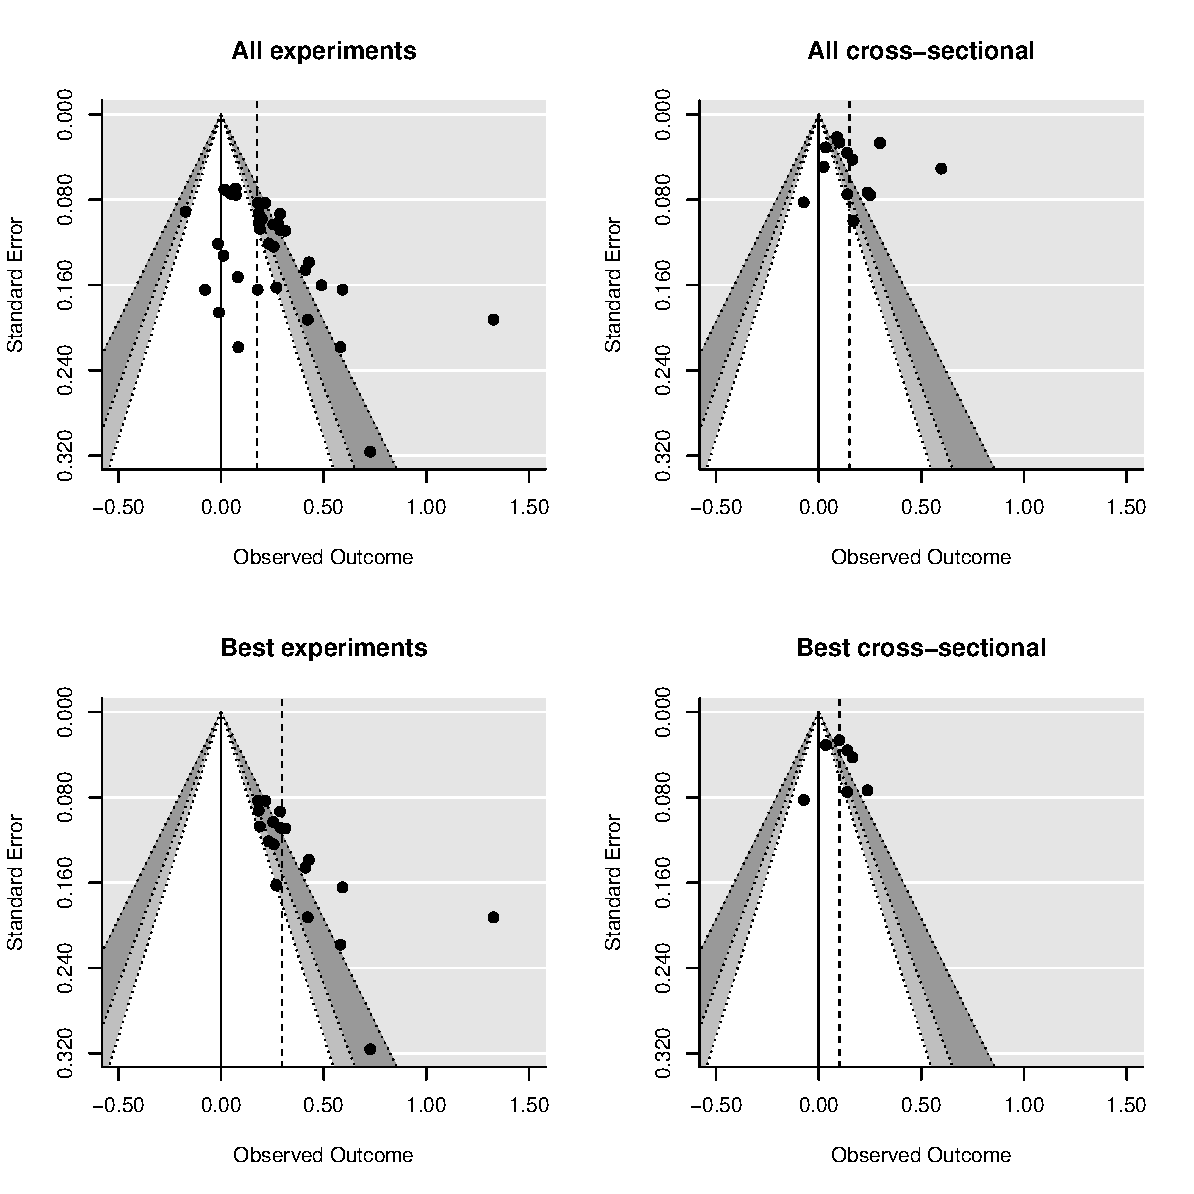
\includegraphics[width = \textwidth, keepaspectratio]{funnels-0_AggAff.pdf}
	\caption{Funnel plot of studies of aggressive affect with shaded contours for $.05 < p < .10$ (light grey) and $.01 < p < .05$ (dark grey). Application of best-practices criteria seems to emphasize statistical significance, and a knot of experiments just reach statistical significance. One best-practices experiment \citep{Ballard:Wiest:1996} finds an implausibly large effect ($z = 1.33$), as does one not-best-practices cross-sectional study \citep[$z = 0.60$]{Urashima:Suzuki:2003}}.
	\label{funnel-aggaff}
\end{figure}

\begin{figure}
	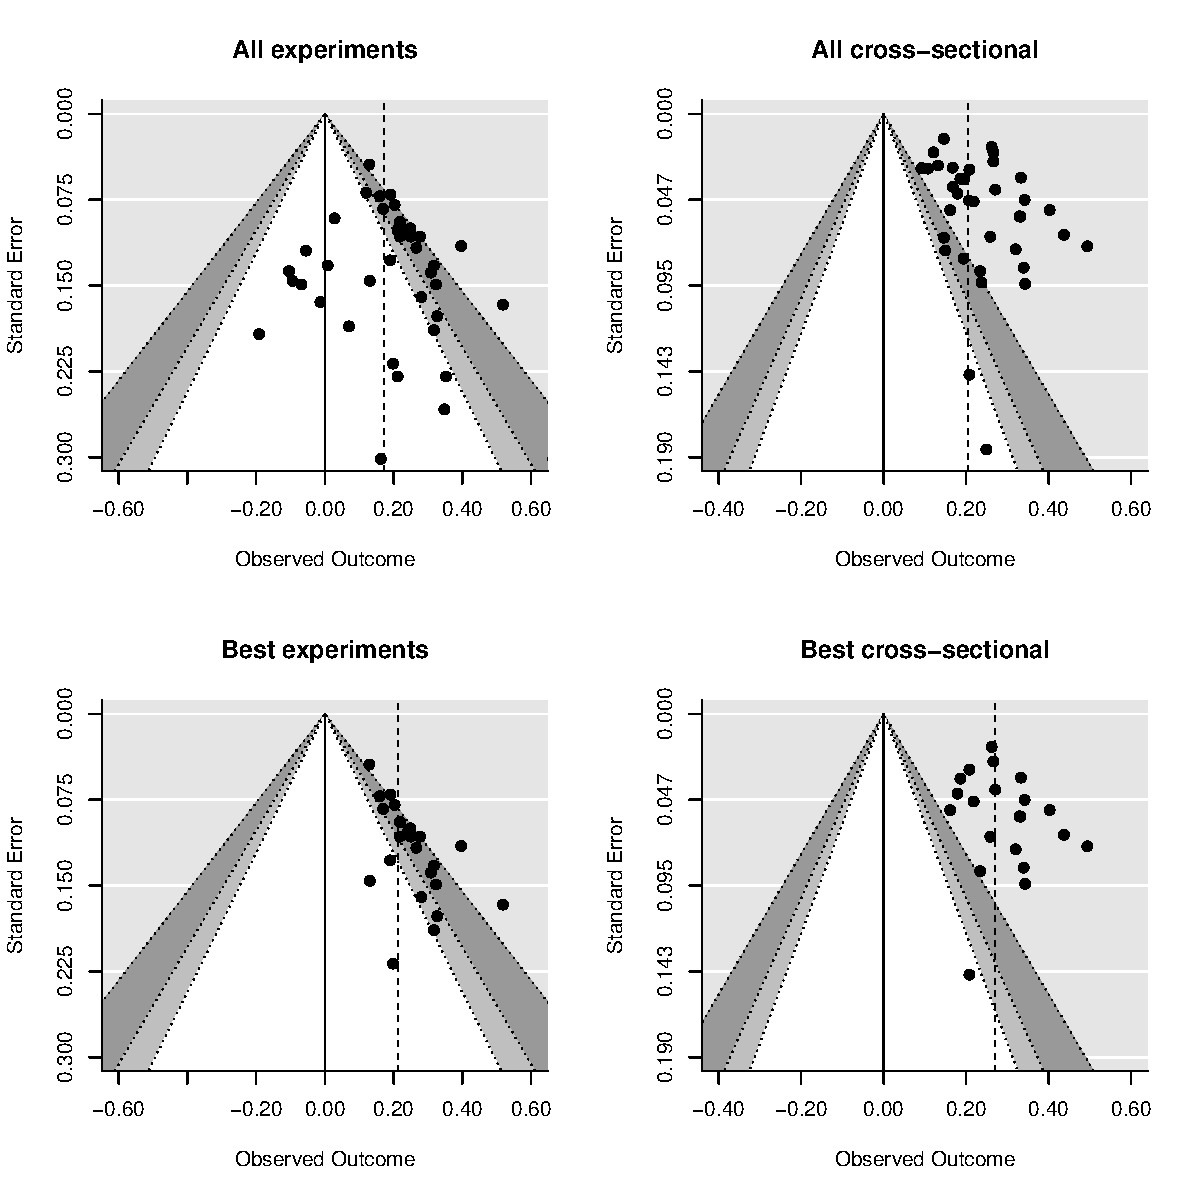
\includegraphics[width = \textwidth, keepaspectratio]{funnels-0_AggBeh.pdf}
	\caption{Funnel plot of studies of aggressive behavior with shaded contours for $.05 < p < .10$ (light grey) and $.01 < p < .05$ (dark grey). Application of best-practices criteria seems to emphasize statistical significance, and a knot of experiments just reach statistical significance. Again, application of best-practices criteria favors experiments finding statistical significance.}
	\label{funnel-aggbeh}
\end{figure}

% TODO: Reviewer 3 points out \citep{Sigurdsson:etal:2006} potential outlier at $z$ = 0.49
\begin{figure}
	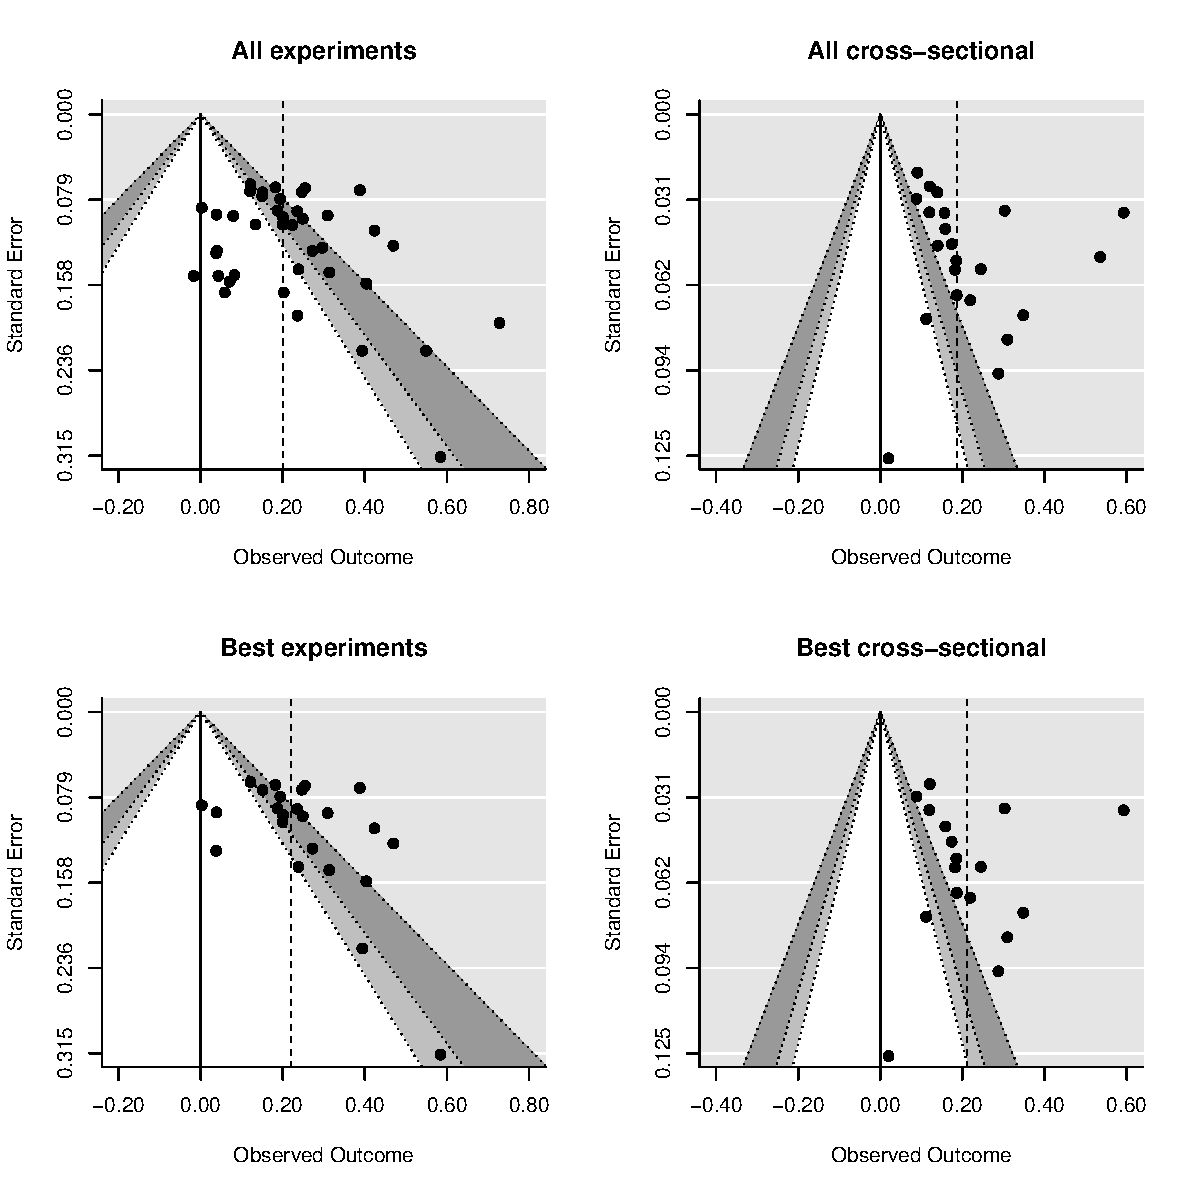
\includegraphics[width = \textwidth, keepaspectratio]{funnels-0_AggCog.pdf}
	\caption{Funnel plot of studies of aggressive cognition with shaded contours for $.05 < p < .10$ (light grey) and $.01 < p < .05$ (dark grey). Results appear moderately heterogeneous, but somewhat less contaminated by bias. One not-best-practices cross-sectional study may be an outlier \citep[$z = 0.49$]{Sigurdsson:etal:2006}.}
	\label{funnel-aggcog}
\end{figure}

\begin{figure}
	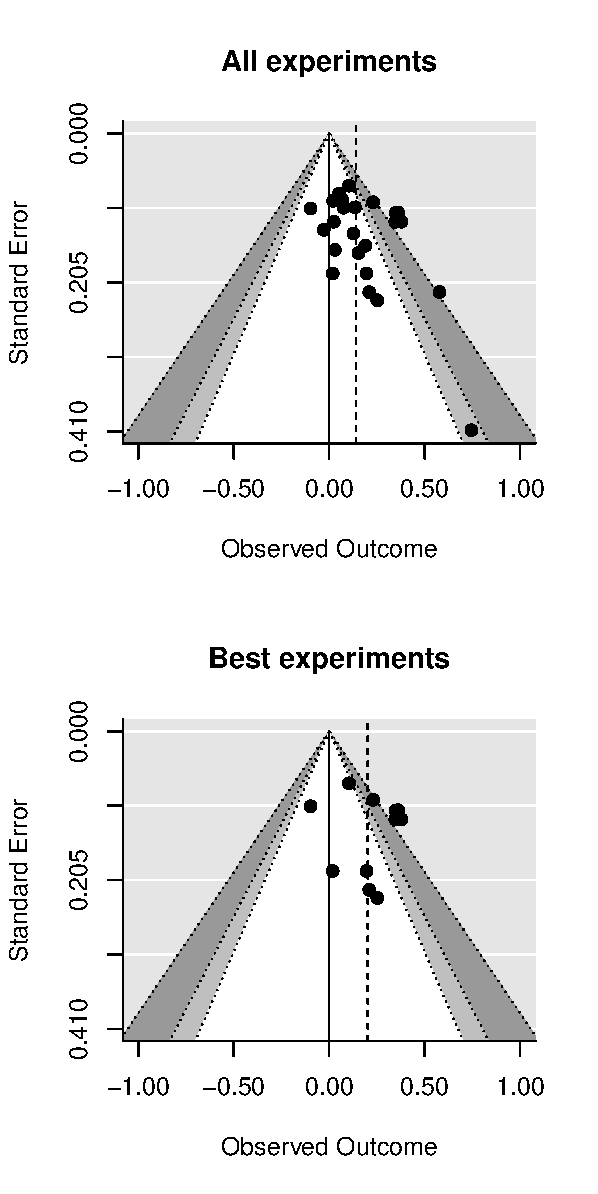
\includegraphics[scale=0.75]{funnels-0_PhysArous.pdf}
	\caption{Funnel plot of studies of physiological arousal with shaded contours for $.05 < p < .10$ (light grey) and $.01 < p < .05$ (dark grey). Application of best-practices criteria seems to emphasize statistical significance, and a knot of experiments just reach statistical significance. Results do not appear to be systematically contaminated by bias.}
	\label{funnel-physarous}
\end{figure}

\begin{figure}
	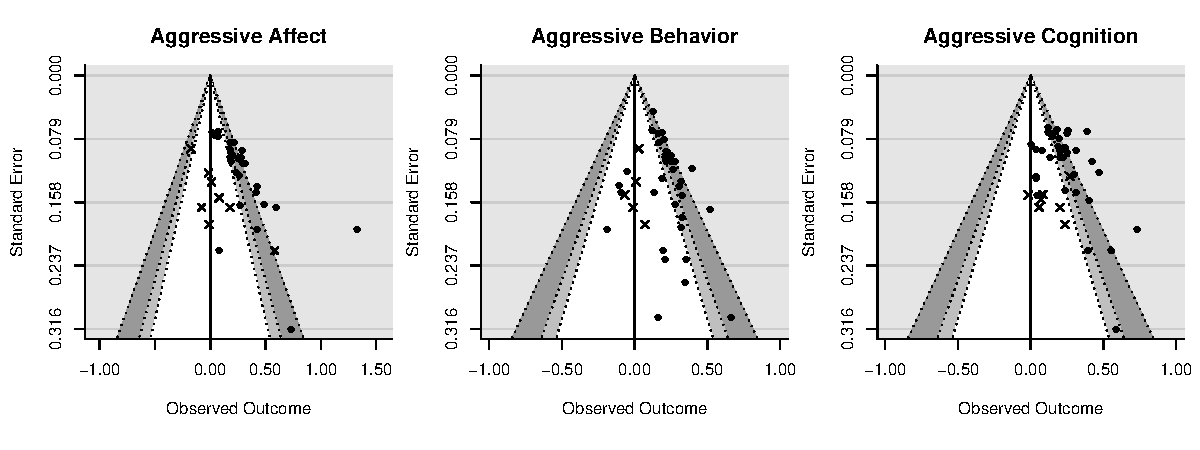
\includegraphics[width = \textwidth, keepaspectratio]{funnel_diss.pdf}
	\caption{Funnel plots of all experiments of aggressive affect, behavior, and cognition. Dissertations not presented in any further publication format are indicated with Xs, while all other publication styles (e.g., journal articles, book chapters, conference proceedings) are indicated with filled dots. Shaded contours represent $p$-values between .10 and .05 (light grey) and between .05 and .01 (dark grey). Nonsignificant results are less likely to be published, and in the case of experimental studies of affect and of behavior, dissertations suggest substantially smaller effects.}
	\label{funnel-diss}
\end{figure}


% Table generated by Excel2LaTeX from sheet 'final_naive'
\begin{table*}[htbp]
	\centering
	\caption{Na{\"i}ve effect-size estimates}
	 \begin{tabular}{ccccccc}
	 	\toprule
	 	&       & \textit{k} & \textit{N} & Fixed & Random & $I^2 (\%)$  \\
	 	\midrule
	 	\multicolumn{7}{c}{Aggressive Affect} \\
	 	Experiment & Best  & 18    & 1318  & .29 [.24, .34] & .34 [.24, .42] & 66 [45, 91] \\
	 	Experiment & Full  & 34    & 2879  & .17 [.14, .21] & .22 [.15, .29] & 72 [61, 89] \\
	 	Cross-Section & Best  & 7     & 4348  & .10 [.07, .13] & .10 [.05, .16] & 65 [12, 96] \\
	 	Cross-Section & Full  & 14    & 9811  & .15 [.13, .17] & .16 [.08, .24] & 93 [87, 98] \\
	 	\multicolumn{7}{c}{Aggressive Behavior} \\
	 	Experiment & Best  & 23    & 2413  & .21 [.17, .25] & .21 [.17, .25] &  4 [0, 17] \\
	 	Experiment & Full  & 39    & 3328  & .17 [.14, .20] & .17 [.14, .20] & 0 [0, 7] \\
	 	Cross-Section & Best  & 21    & 11615 & .26 [.25, .28] & .28 [.24, .31] & 67 [38, 86] \\
	 	Cross-Section & Full  & 36    & 28337 & .20 [.19, .21] & .23 [.20, .26] & 82 [70, 90] \\
	 	\multicolumn{7}{c}{Aggressive Cognition} \\
	 	Experiment & Best  & 24    & 2887  & .22 [.18, .25] & .22 [.18, .27] & 35 [0, 70] \\
	 	Experiment & Full  & 40    & 4073.5 & .20 [.17, .23] & .20 [.16, .24] & 27 [0, 67] \\
	 	Cross-Section & Best  & 16    & 7221  & .17 [.15, .19] & .18 [.14, .22] & 62 [27, 85] \\
	 	Cross-Section & Full  & 21    & 12236 & .16 [.14, .18] & .19 [.14, .24] & 84 [70, 93] \\
	 	\multicolumn{7}{c}{Physiological Arousal} \\
	 	Experiment & Best  & 11    & 833   & .20 [.13, .26] & .21 [.11, .31] & 50 [0, 80] \\
	 	Experiment & Full  & 24    & 1770  & .14 [.09, .18] & .15 [.09, .21] & 35 [0, 71] \\
	 	\bottomrule
	 \end{tabular}%
	\label{table:naive}%
	\caption*{Note: K = {\em number of studies;} N = {\em total N across studies. All effect sizes in Pearson $r$ with 95\% confidence intervals.}}
\end{table*}%

% Table generated by Excel2LaTeX from sheet 'Egger test'
\begin{table*}[htbp]
	\centering
	\caption{Tests for bias and small-study effects.}
	\begin{tabular}{cccccccc}
		\toprule
		Outcome & Setting & Best  & $b_{Egger}$ & SE($b_{Egger}$) & $p_{Egger}$ & $p_{p-uniform}$ & $p_{TES}$ \\
		\midrule
		Affect & Experiment & Best  & 3.667 & 0.78  & \textbf{< .001} & 0.201 & 0.079 \\
		Affect & Experiment & Full  & 2.635 & 0.737 & \textbf{< .001} & 0.861 & \textbf{0.022} \\
		Affect & Cross-Section & Best  & -     & -     & -     & -     & - \\
		Affect & Cross-Section & Full  & 0.123 & 1.883 & 0.948 & 0.661 & 0.211 \\
		Behavior & Experiment & Best  & 1.537 & 0.549 & \textbf{0.005} & \textbf{0.002} & \textbf{0.015} \\
		Behavior & Experiment & Full  & 0.451 & 0.39  & 0.248 & \textbf{0.009} & \textbf{0.020} \\
		Behavior & Cross-Section & Best  & 1.163 & 0.789 & 0.140  & 0.752 & 0.931 \\
		Behavior & Cross-Section & Full  & 1.326 & 0.589 & \textbf{0.024} & 0.900   & 0.199 \\
		Cognition & Experiment & Best  & 1.372 & 0.761 & 0.071 & 0.684 & 0.309 \\
		Cognition & Experiment & Full  & 0.883 & 0.544 & 0.104 & 0.814 & 0.339 \\
		Cognition & Cross-Section & Best  & 1.061 & 0.941 & 0.259 & 0.628 & 0.354 \\
		Cognition & Cross-Section & Full  & 1.241 & 1.064 & 0.243 & 0.544 & 0.234 \\
		Arousal & Experiment & Best  & 0.137 & 1.22  & 0.911 & 0.797 & 0.636 \\
		Arousal & Experiment & Full  & 1.295 & 0.714 & 0.070  & 0.93  & 0.704 \\
		\bottomrule
	\end{tabular}%
	\label{table:Egger}%
	\caption*{Note: {\em One analysis omitted for insufficient number of studies. Bold text highlights significant test results.
			%One may also consider $\alpha = .008$ as the threshold for significance, based on a combination of Egger's recommendation of $\alpha = .10$ and 13-fold Bonferroni correction.
			}}
\end{table*}%

% Table generated by Excel2LaTeX from sheet 'adjustment_jeffstyle'
\begin{table*}[htbp]
	\small
	\centering
	\caption{Adjusted effect-size estimates.}
	\begin{tabular}{rrrrrrrr}
		\toprule
		&       & PET   & $I^2_{PET} (\%)$ & PEESE & $I^2_{PEESE} (\%)$ & $p$-uniform & $p$-curve \\
		\midrule
		\multicolumn{8}{c}{Aggressive Affect} \\
		Experiment & Best  & -.12 [-.29, .06] & 0 [0, 83] & .14 [.06, .23] &  0 [0, 86] & .24 [.08, .36] & .21 \\
		Experiment & Full  & -.10 [-.27, .08] & 58 [44, 85] & .08 [-.02, .18] & 60 [47, 86] & .24 [.11, .35] & .20 \\
		Cross-Section & Best  & -     & -     & -     & -     & -     & - \\
		Cross-Section & Full  &  .16 [-.04, .35] & 94 [88, 98] & .17 [.04, .29] & 94 [88, 98] & .16 [.12, .24] & .16 \\
		\multicolumn{8}{c}{Aggressive Behavior} \\
		Experiment & Best  &  .07 [-.04, .18] &  0 [$\dagger$] & .15 [.09, .21] &  0 [$\dagger$] & .02 [-.23, .15] & .09 \\
		Experiment & Full  &  \textbf{.13 [.04, .21]} & 0 [0, 7] & .15 [.10, .20] & 0 [0, 7] & .02 [-.23, .15] & .08 \\
		Cross-Section & Best  &  .22 [.14, .30] & 62 [30, 86] & .26 [.21, .30] & 65 [35, 87] & .27 [.24, .31] & .27 \\
		Cross-Section & Full  &  .17 [.11, .23] & 79 [65, 89] & .21 [.18, .25] & 81 [69, 90] & .22 [.19, .25] & .23 \\
		\multicolumn{8}{c}{Aggressive Cognition} \\
		Experiment & Best  &  .10 [-.05, .24] & 33 [0, 65] & .18 [.11, .24] & 32 [0, 65] & .24 [.15, .31] & .19 \\
		Experiment & Full  &  \textbf{.11 [.00, .22]} & 29 [0, 64] & .16 [.10, .21] & 27 [0, 62] & .24 [.14, .32] & .19 \\
		Cross-Section & Best  &  \textbf{.13 [.03, .23]} & 58 [22, 87] & .17 [.11, .23] & 61 [26, 87] & .18 [.14, .22] & .17 \\
		Cross-Section & Full  &  \textbf{.13 [.02, .24]} & 82 [68, 93] & .18 [.11, .24] & 84 [71, 93] & .16 [.13, .20] & .17 \\
		\multicolumn{8}{c}{Physiological Arousal} \\
		Experiment & Best  &  .19 [-.12, .47] & 53 [0, 83] & .21 [.04, .37] & 54 [0, 84] & .26 [.08, .37] & .28 \\
		Experiment & Full  & -.01 [-.18, .17] & 31 [0, 66] & .09 [.00, .17] & 32 [0, 65] & .26 [.08, .37] & .28 \\
		\bottomrule
	\end{tabular}%
	\label{table:adjustment}%
	\caption*{Note: K = {\em number of studies;} N = {\em total N across studies. $\dagger$ Confidence interval on $I^2$ unavailable due to highly homogeneous data. One analysis omitted for insufficient number of studies. Bold text indicates where the $95\%$ CI of the PET estimate excludes zero, suggesting that the underlying effect is nonzero and that PEESE should be favored over PET. All effect sizes in Pearson $r$.}}
\end{table*}%

% Table generated by Excel2LaTeX from sheet 'dissertation_freqtable'
\begin{table*}[htbp]
	\small
	\centering
	\caption{The statistical significance and best-practices coding of effect sizes in unpublished dissertations.}
	\begin{tabular}{rrrr}
		\toprule
		\multicolumn{3}{c}{\textbf{Liberal coding scheme.}} &  \\
		\midrule
		& \multicolumn{2}{c}{Statistical significance} &  \\
		Publication format & Yes   & No    &  \\
		Unpublished Dissertation & 4     & 30    &  \\
		Other & 199   & 125   &  \\
		&       &       &  \\
		& \multicolumn{2}{c}{Labeled Best Practices} &  \\
		Publication format & Yes   & No    &  \\
		Unpublished Dissertation & 4     & 30    &  \\
		Other & 206   & 118   &  \\
		&       &       &  \\
		\multicolumn{4}{c}{\textbf{Conservative coding scheme.}} \\
		& \multicolumn{3}{c}{Statistical significance} \\
		Publication format & All outcomes   & Some outcomes & No outcomes \\
		Unpublished Dissertation & 2     & 2     & 14 \\
		Other & 72    & 34    & 29 \\
		&       &       &  \\
		& \multicolumn{2}{c}{Labeled Best Practices} &  \\
		Publication format & Yes   & No    &  \\
		Unpublished Dissertation & 3     & 15    &  \\
		Other & 82    & 62    &  \\
		\bottomrule
	\end{tabular}%
	\label{table:dissertations}%
\end{table*}

\end{document}